\documentclass[12pt]{article}
\usepackage[margin=2.5cm]{geometry}
\usepackage{enumerate}
\usepackage{amsfonts}
\usepackage{amsmath}
\usepackage{fancyhdr}
\usepackage{amsmath}
\usepackage{amssymb}
\usepackage{amsthm}
\usepackage{mdframed}
\usepackage{graphicx}
\usepackage{subcaption}
\usepackage{adjustbox}
\usepackage{listings}
\usepackage{xcolor}
\usepackage{booktabs}
\usepackage[utf]{kotex}
\usepackage{hyperref}

\definecolor{codegreen}{rgb}{0,0.6,0}
\definecolor{codegray}{rgb}{0.5,0.5,0.5}
\definecolor{codepurple}{rgb}{0.58,0,0.82}
\definecolor{backcolour}{rgb}{0.95,0.95,0.92}

\lstdefinestyle{mystyle}{
    backgroundcolor=\color{backcolour},
    commentstyle=\color{codegreen},
    keywordstyle=\color{magenta},
    numberstyle=\tiny\color{codegray},
    stringstyle=\color{codepurple},
    basicstyle=\ttfamily\footnotesize,
    breakatwhitespace=false,
    breaklines=true,
    captionpos=b,
    keepspaces=true,
    numbers=left,
    numbersep=5pt,
    showspaces=false,
    showstringspaces=false,
    showtabs=false,
    tabsize=1
}

\lstset{style=mystyle}

\pagestyle{fancy}
\renewcommand{\headrulewidth}{0.4pt}
\lhead{CSC 343}
\rhead{Worksheet 1}

\begin{document}
\title{CSC343 Worksheet 1}
\maketitle

\noindent \textbf{Note:} This is student designed study guide to make learnings easier.
This does not reflect the course material. Please take it only as a reference.

\begin{enumerate}[1.]
    \item \textbf{Exercise 2.2.1:} In fig 2.6 are instances of two relations that might
    constitute part of a banking exercise. Indicate the following

    \begin{center}
    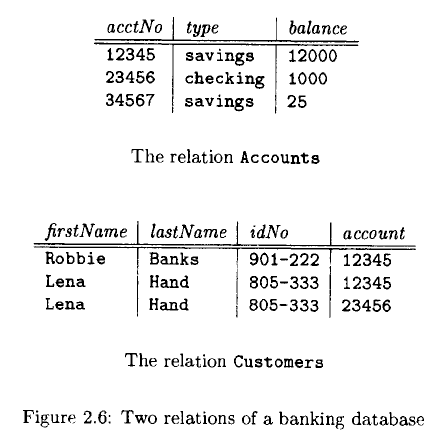
\includegraphics[width=\linewidth]{images/worksheet_1_1.png}
    \end{center}

    \begin{enumerate}[a)]
        \item The attributes of each relation
        \item The tuples of each relation
        \item The components of one tuple from each relation
        \item The database schema
        \item A suitable domain for each attribute
        \item Another equivalent way to present each relation
    \end{enumerate}

    \item \textbf{Exercise 2.2.2:} In section 2.2.7 we suggested that there are many
    exmaples of attributes that are created for the purpose of serving as keys of
    relations. Give some additional examples.


    \item \textbf{Exericse 2.3.1} In this exercise we introduce one of our running
    examples of a relational database schema. The database schema consists of four relations,
    whose schemas are:

    \bigskip

    \begin{lstlisting}
    Product(maker, model, type)
    PC(model, speed, ram, hd, price)
    Laptop(model, speed, ram, hd, screen, price)
    Printer(model, color, type, price)
    \end{lstlisting}
\end{enumerate}

\bigskip

\underline{\textbf{Reference}}

\bigskip

\begin{enumerate}[1)]
    \item Stanford: CS145 - Introduction to Databases, \href{http://infolab.stanford.edu/~ullman/fcdb/aut07/index.html}{link}
\end{enumerate}

\end{document}